\chapter{RELEASE 2}
\addcontentsline{toc}{chapter}{Chapitre 4 : RELEASE 2}

\section*{Introduction}
\addcontentsline{toc}{section}{Introduction}
Dans ce chapitre, nous explorerons en détail le deuxième release de notre projet, qui contient la troisième sprint.

\section{Organisation du sprint}
Notre release est composée par :\\
\textbf{- Sprint 3 :} Gestion des événements (CRUD).

\section{Sprint 3 : Gestion des événements (CRUD)}
\subsection{Objectif du sprint}
L'objectif de ce sprint est la création, modification, suppression et affichage des événements. Les tâches principales sont :
\begin{itemize}
    \item Implémentation des routes backend pour événements
    \item Création du modèle événement
    \item Validation des champs d'événements
    \item Affichage dynamique des événements
\end{itemize}

\subsection{Sprint backlog}
Le 3ème sprint s'étend du 22 février au 04 mars. Le tableau suivant représente le backlog de ce sprint:

\begin{table}[h!]
\renewcommand{\arraystretch}{1.6}
\setlength{\tabcolsep}{5pt}
\centering
\begin{tabular}{|c|c|m{7cm}|c|c|}
\hline
\textbf{ID} & \textbf{Sprint} & \textbf{User Story} & \textbf{Priorité} & \textbf{Complexité} \\
\hline
3 & \parbox{3cm}{\centering Gestion des\\ événements} & En tant qu'administrateur, je veux modifier des événements. & Élevée & Moyenne \\
\hline
3 & \parbox{3cm}{\centering Gestion des\\ événements} & En tant qu'administrateur, je veux supprimer des événements. & Élevée & Moyenne \\
\hline
3 & \parbox{3cm}{\centering Gestion des\\ événements} & En tant qu'administrateur, je veux consulter des événements. & Élevée & Moyenne \\
\hline
3 & \parbox{3cm}{\centering Gestion des\\ événements} & En tant qu'administrateur, je veux approuver des événements. & Élevée & Moyenne \\
\hline
3 & \parbox{3cm}{\centering Gestion des\\ événements} & En tant que gestionnaire, je veux créer des événements. & Élevée & Moyenne \\
\hline
3 & \parbox{3cm}{\centering Gestion des\\ événements} & En tant que gestionnaire, je veux modifier des événements. & Élevée & Moyenne \\
\hline
3 & \parbox{3cm}{\centering Gestion des\\ événements} & En tant que gestionnaire, je veux supprimer des événements. & Élevée & Moyenne \\
\hline
\end{tabular}
\caption{User Stories - Sprint Gestion des événements}
\end{table}

\subsection{Implémentation du sprint 3}
\subsubsection{Spécification des besoins}
Dans cette section, nous identifions les besoins de notre sprint, à travers :
\begin{itemize}
    \item les diagrammes de cas d'utilisation,
    \item les descriptions textuelles associées,
    \item les diagrammes de séquences système.
\end{itemize}

\textbf{La figure ci-dessous représente le diagramme de cas d'utilisation de ce sprint par rapport à l'administrateur.}

\begin{figure}[H]
    \centering
    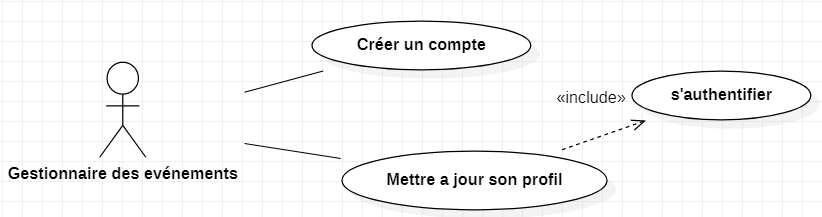
\includegraphics[width=0.6\linewidth]{projet/images/diagramme de sequance/images/gestionnaire.png}
    \caption{Diagramme des cas d'utilisation gestion d'événement "Administrateur"}
    \label{fig:AdminEvent}
\end{figure}

Ce diagramme décrit le processus de gestion d'événement pour l'administrateur. Nous détaillons ci-après ce cas d'utilisation sous forme textuelle :